%package list
\documentclass{article}
\usepackage[top=3cm, bottom=3cm, outer=3cm, inner=3cm]{geometry}
\usepackage{multicol}
\usepackage{graphicx}
\usepackage{url}
%\usepackage{cite}
\usepackage{hyperref}
\usepackage{array}
%\usepackage{multicol}
\newcolumntype{x}[1]{>{\centering\arraybackslash\hspace{0pt}}p{#1}}
\usepackage{natbib}
\usepackage{pdfpages}
\usepackage{multirow}
\usepackage[normalem]{ulem}
\useunder{\uline}{\ul}{}
\usepackage{svg}
\usepackage{xcolor}
\usepackage{listings}
\lstdefinestyle{ascii-tree}{
    literate={├}{|}1 {─}{--}1 {└}{+}1 
}
\lstset{frame=tb,
language=bash,
aboveskip=3mm,
belowskip=3mm,
showstringspaces=false,
columns=flexible,
basicstyle={\small\ttfamily},
numbers=none,
numberstyle=\tiny\color{gray},
keywordstyle=\color{blue},
commentstyle=\color{dkgreen},
stringstyle=\color{mauve},
breaklines=true,
breakatwhitespace=true,
tabsize=3,
backgroundcolor= \color{codebackground},
literate={á}{{\'a}}1 {é}{{\'e}}1 {í}{{\'i}}1 {ó}{{\'o}}1 {ú}{{\'u}}1 {Á}{{\'A}}1 {É}{{\'E}}1 {Í}{{\'I}}1 {Ó}{{\'O}}1 {Ú}{{\'U}}1 {ñ}{{\~n}}1
}
%\usepackage{booktabs}
\usepackage[labelformat=empty]{caption}
\usepackage{subcaption}
\usepackage{float}
\usepackage{array}

\newcolumntype{M}[1]{>{\centering\arraybackslash}m{#1}}
\newcolumntype{N}{@{}m{0pt}@{}}


%%%%%%%%%%%%%%%%%%%%%%%%%%%%%%%%%%%%%%%%%%%%%%%%%%%%%%%%%%%%%%%%%%%%%%%%%%%%
%%%%%%%%%%%%%%%%%%%%%%%%%%%%%%%%%%%%%%%%%%%%%%%%%%%%%%%%%%%%%%%%%%%%%%%%%%%%
\newcommand{\itemEmail}{cmestasz@unsa.edu.pe}
\newcommand{\itemStudent}{Christian Mestas Zegarra}
\newcommand{\itemCourse}{Fundamentos de la Programación 2}
\newcommand{\itemCourseCode}{1701213}
\newcommand{\itemSemester}{II}
\newcommand{\itemUniversity}{Universidad Nacional de San Agustín de Arequipa}
\newcommand{\itemFaculty}{Facultad de Ingeniería de Producción y Servicios}
\newcommand{\itemDepartment}{Departamento Académico de Ingeniería de Sistemas e Informática}
\newcommand{\itemSchool}{Escuela Profesional de Ingeniería de Sistemas}
\newcommand{\itemAcademic}{2023 - B}
\newcommand{\itemInput}{Del 22 Enero 2024}
\newcommand{\itemOutput}{Al 29 Enero 2024}
\newcommand{\itemPracticeNumber}{Proyecto Final}
\newcommand{\itemTheme}{Proyecto Final}
%%%%%%%%%%%%%%%%%%%%%%%%%%%%%%%%%%%%%%%%%%%%%%%%%%%%%%%%%%%%%%%%%%%%%%%%%%%%
%%%%%%%%%%%%%%%%%%%%%%%%%%%%%%%%%%%%%%%%%%%%%%%%%%%%%%%%%%%%%%%%%%%%%%%%%%%%

\usepackage[english,spanish]{babel}
\usepackage[utf8]{inputenc}
\AtBeginDocument{\selectlanguage{spanish}}
\renewcommand{\figurename}{Figura}
\renewcommand{\refname}{Referencias}
\renewcommand{\tablename}{Tabla} %esto no funciona cuando se usa babel
\AtBeginDocument{%
	\renewcommand\tablename{Tabla}
}

\usepackage{fancyhdr}
\pagestyle{fancy}
\fancyhf{}
\setlength{\headheight}{30pt}
\renewcommand{\headrulewidth}{1pt}
\renewcommand{\footrulewidth}{1pt}
\fancyhead[L]{\raisebox{-0.2\height}{
\includegraphics[width=3cm]{img/logo_episunsa.png}}}
\fancyhead[C]{\fontsize{7}{7}\selectfont	\itemUniversity \\ \itemFaculty \\ \itemDepartment \\ \itemSchool \\ \textbf{\itemCourse}}
\fancyhead[R]{\raisebox{-0.2\height}{
\includegraphics[width=1.2cm]{img/logo_abet}}}
\fancyfoot[L]{Christian Mestas}
\fancyfoot[C]{\itemCourse}
\fancyfoot[R]{Página \thepage}

% para el codigo fuente
\usepackage{listings}
\usepackage{color, colortbl}
\definecolor{dkgreen}{rgb}{0,0.6,0}
\definecolor{gray}{rgb}{0.5,0.5,0.5}
\definecolor{mauve}{rgb}{0.58,0,0.82}
\definecolor{codebackground}{rgb}{0.95, 0.95, 0.92}
\definecolor{tablebackground}{rgb}{0.8, 0, 0}

\lstset{frame=tb,
	language=bash,
	aboveskip=3mm,
	belowskip=3mm,
	showstringspaces=false,
	columns=flexible,
	basicstyle={\small\ttfamily},
	numbers=none,
	numberstyle=\tiny\color{gray},
	keywordstyle=\color{blue},
	commentstyle=\color{dkgreen},
	stringstyle=\color{mauve},
	breaklines=true,
	breakatwhitespace=true,
	tabsize=3,
	backgroundcolor= \color{codebackground},
}

\begin{document}

\vspace*{10px}

\begin{center}
	\fontsize{17}{17} \textbf{ Informe de Laboratorio \itemPracticeNumber}
\end{center}
\centerline{\textbf{\Large Tema: \itemTheme}}
%\vspace*{0.5cm}	

\begin{flushright}
	\begin{tabular}{|M{2.5cm}|N|}
		\hline
		\rowcolor{tablebackground}
		\color{white} \textbf{Nota} \\
		\hline
		\\[30pt]
		\hline
	\end{tabular}
\end{flushright}

\begin{table}[H]
	\begin{tabular}{|M{4.7cm}|M{4.8cm}|M{4.8cm}|}
		\hline
		\rowcolor{tablebackground}
		\color{white} \textbf{Estudiante} & \color{white}\textbf{Escuela} & \color{white}\textbf{Asignatura}                                        \\
		\hline
		{\itemStudent \par \itemEmail}    & \itemSchool                   & {\itemCourse \par Semestre: \itemSemester \par Código: \itemCourseCode} \\
		\hline
	\end{tabular}
\end{table}

\begin{table}[H]
	\begin{tabular}{|M{4.7cm}|M{4.8cm}|M{4.8cm}|}
		\hline
		\rowcolor{tablebackground}
		\color{white}\textbf{Laboratorio} & \color{white}\textbf{Tema} & \color{white}\textbf{Duración} \\
		\hline
		\itemPracticeNumber               & \itemTheme                 & 04 horas                       \\
		\hline
	\end{tabular}
\end{table}

\begin{table}[H]
	\begin{tabular}{|M{4.7cm}|M{4.8cm}|M{4.8cm}|}
		\hline
		\rowcolor{tablebackground}
		\color{white}\textbf{Semestre académico} & \color{white}\textbf{Fecha de inicio} & \color{white}\textbf{Fecha de entrega} \\
		\hline
		\itemAcademic                            & \itemInput                            & \itemOutput                            \\
		\hline
	\end{tabular}
\end{table}

%%%%%%%%%%%%%%%%%%%%%%%%%%%%%%%%%%%%%%%%%%%%%%%%%%%%%%%%%%%%%%%%%%%%%%
\section{Tarea}
\begin{itemize}
	\item \textbf{Enunciado:}
	      \\• Cree una versión del videojuego de estrategia usando componentes de GUI, bases de datos y archivos.
\end{itemize}
%%%%%%%%%%%%%%%%%%%%%%%%%%%%%%%%%%%%%%%%%%%%%%%%%%%%%%%%%%%%%%%%%%%%%%
\pagebreak

\section{Equipos, materiales y temas utilizados}
\begin{itemize}
	\item Sistema Operativo Microsoft Windows 10 Pro 64 bits
	\item Visual Studio Code 1.82.2
	\item Java Development Kit 17.0.1
	\item JavaFX sdk 21.0.1
	\item Git 2.41.0.windows.1
	\item Windows PowerShell 5.1.19041.3031
	\item Cuenta en GitHub con el correo institucional.
	      %%%%%%%%%%%%%%%%%%%%%%%%%%%%%%%%%%%%%%%%%%%%%%%%%%%%%%%%%%%%%%%%%%%%%%
	\item Programación Orientada a Objetos
	\item HashMap de Objetos
	\item Agregación y composición
	\item Herencia y polimorfismo
	\item Interfaces
	\item Miembros de clase e instancia
	\item Interfaz gráfica de usuario
	\item Bases de datos
	\item Archivos
	      %%%%%%%%%%%%%%%%%%%%%%%%%%%%%%%%%%%%%%%%%%%%%%%%%%%%%%%%%%%%%%%%%%%%%%
\end{itemize}

\section{URL de Repositorio Github}
\begin{itemize}
	\item URL del Repositorio GitHub para clonar o recuperar.
	\item \url{https://github.com/cmestasz/fp2-23b.git}
	      %%%%%%%%%%%%%%%%%%%%%%%%%%%%%%%%%%%%%%%%%%%%%%%%%%%%%%%%%%%%%%%%%%%%%%
	\item URL del proyecto final en el Repositorio GitHub.
	\item \url{https://github.com/cmestasz/fp2-23b/tree/main/fase03/proyecto_final}
	      %%%%%%%%%%%%%%%%%%%%%%%%%%%%%%%%%%%%%%%%%%%%%%%%%%%%%%%%%%%%%%%%%%%%%%
\end{itemize}
\pagebreak

\section{Actividades con el repositorio GitHub}
\lstinputlisting[keepspaces=true,language=bash,caption={commits.bash},numbers=left,]{commits.bash}
\begin{figure}[H]
	\centering
	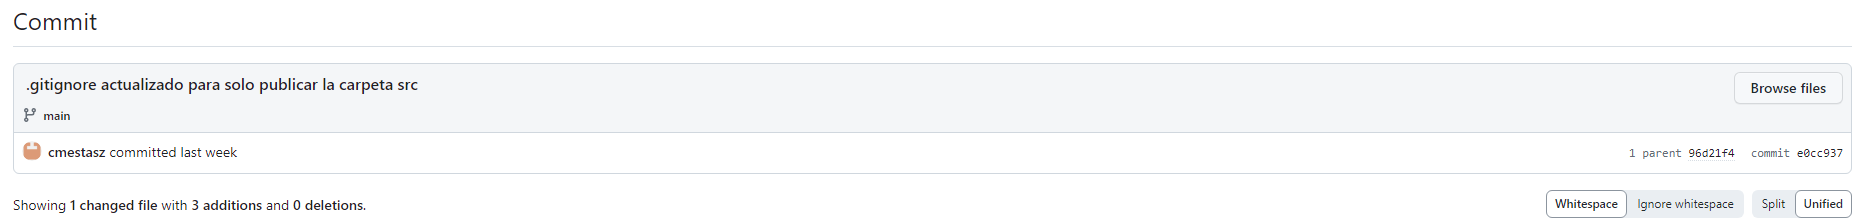
\includegraphics[width=1\textwidth,keepaspectratio]{img/commit_01.png}
	\caption{.gitignore actualizado para solo publicar la carpeta src}
\end{figure}
\begin{figure}[H]
	\centering
	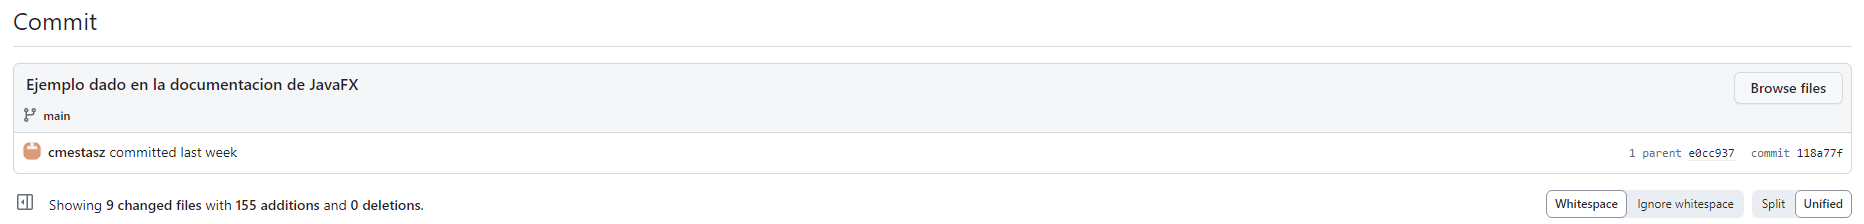
\includegraphics[width=1\textwidth,keepaspectratio]{img/commit_02.png}
	\caption{Ejemplo dado en la documentacion de JavaFX}
\end{figure}
\begin{figure}[H]
	\centering
	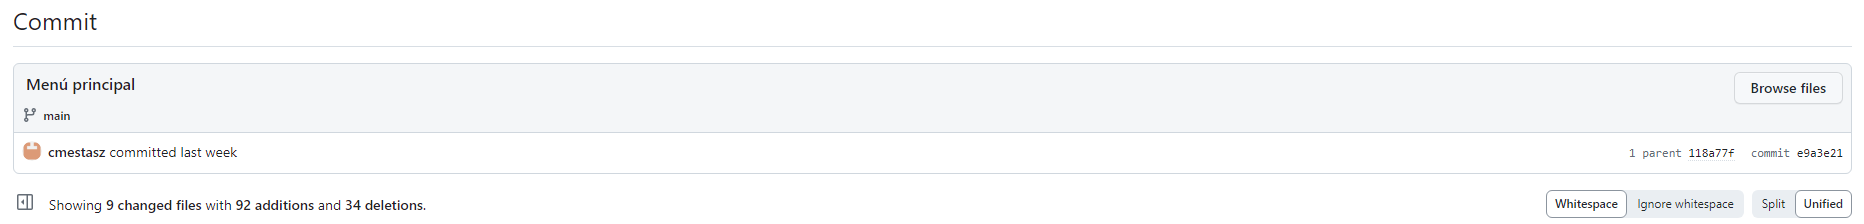
\includegraphics[width=1\textwidth,keepaspectratio]{img/commit_03.png}
	\caption{Menú principal}
\end{figure}
\begin{figure}[H]
	\centering
	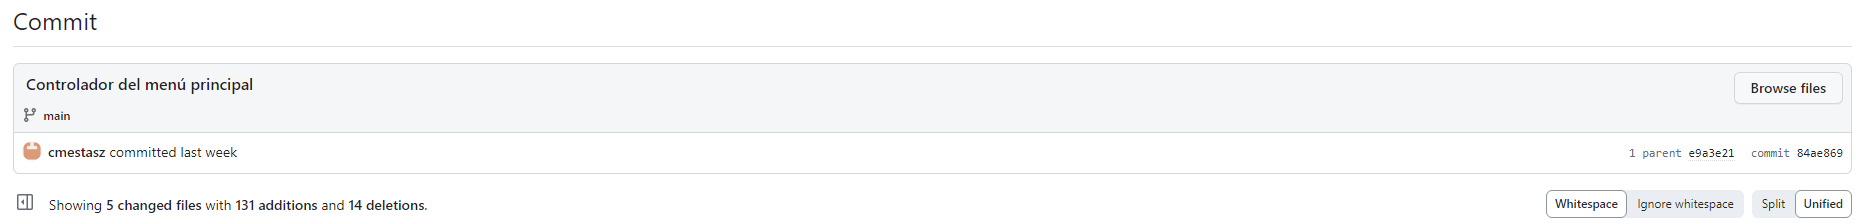
\includegraphics[width=1\textwidth,keepaspectratio]{img/commit_04.png}
	\caption{Controlador del menú principal}
\end{figure}
\begin{figure}[H]
	\centering
	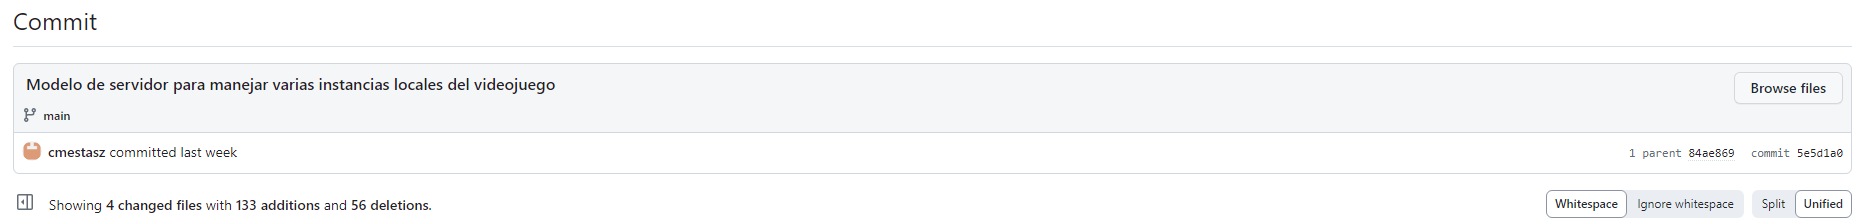
\includegraphics[width=1\textwidth,keepaspectratio]{img/commit_05.png}
	\caption{Modelo de servidor para manejar varias instancias locales del videojuego}
\end{figure}
\begin{figure}[H]
	\centering
	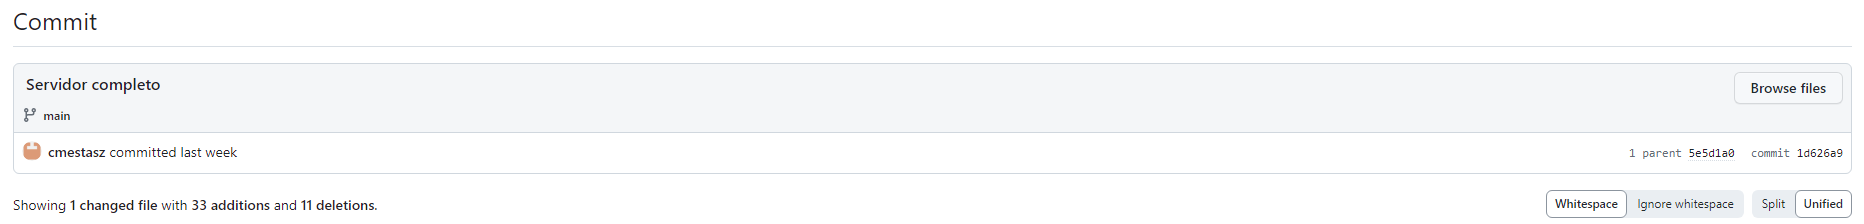
\includegraphics[width=1\textwidth,keepaspectratio]{img/commit_06.png}
	\caption{Servidor completo}
\end{figure}
\begin{figure}[H]
	\centering
	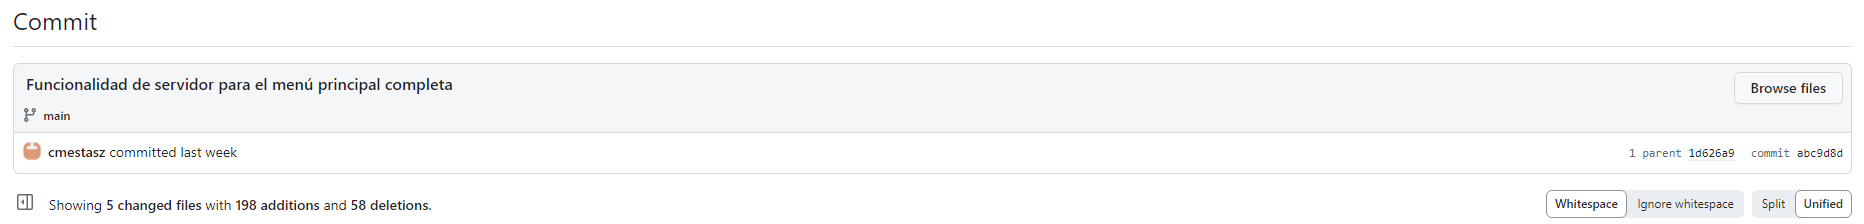
\includegraphics[width=1\textwidth,keepaspectratio]{img/commit_07.png}
	\caption{Funcionalidad de servidor para el menú principal completa}
\end{figure}
\begin{figure}[H]
	\centering
	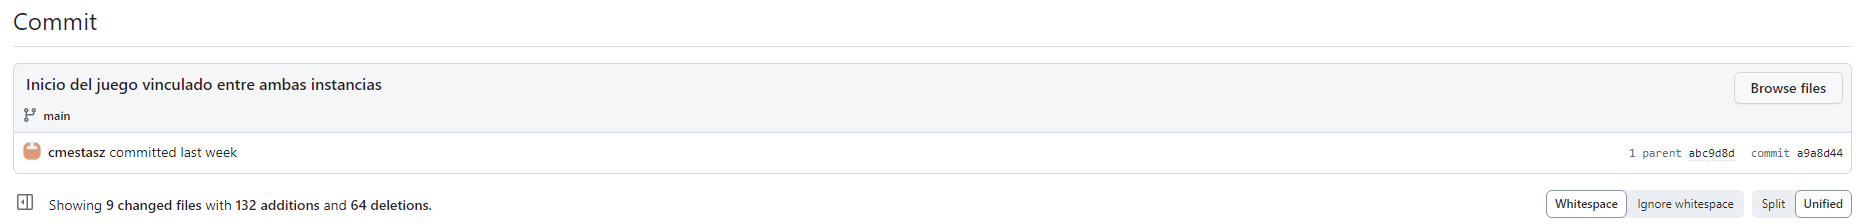
\includegraphics[width=1\textwidth,keepaspectratio]{img/commit_08.png}
	\caption{Inicio del juego vinculado entre ambas instancias}
\end{figure}
\begin{figure}[H]
	\centering
	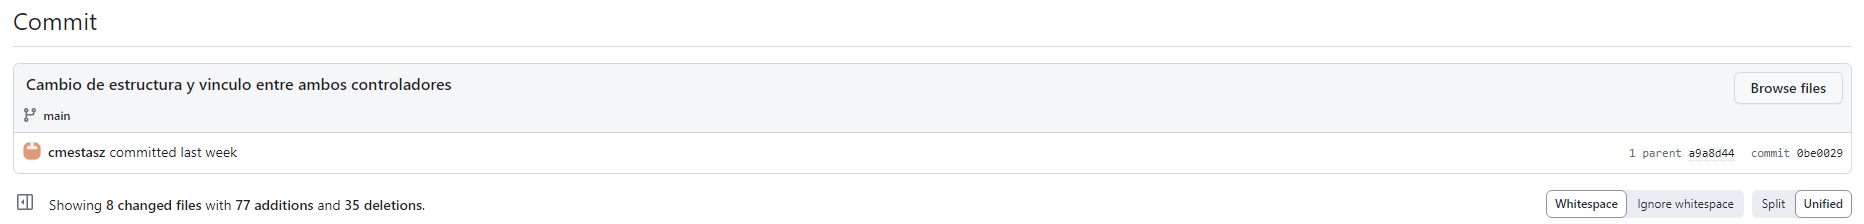
\includegraphics[width=1\textwidth,keepaspectratio]{img/commit_09.png}
	\caption{Cambio de estructura y vinculo entre ambos controladores}
\end{figure}
\begin{figure}[H]
	\centering
	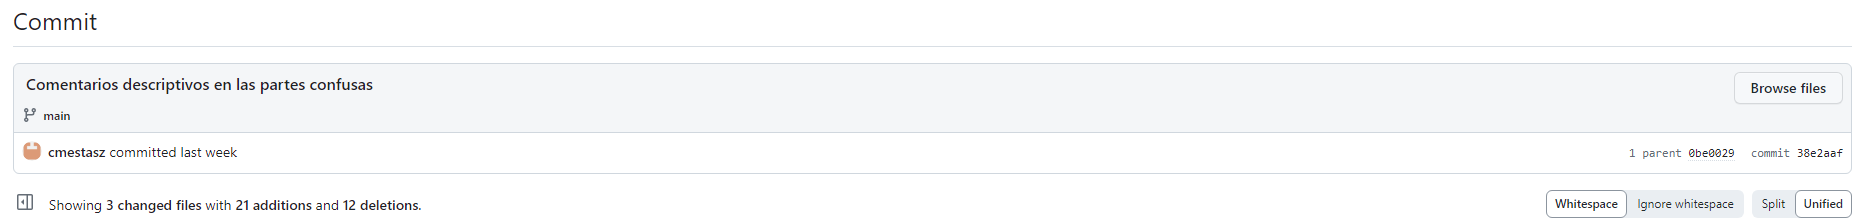
\includegraphics[width=1\textwidth,keepaspectratio]{img/commit_10.png}
	\caption{Comentarios descriptivos en las partes confusas}
\end{figure}
\begin{figure}[H]
	\centering
	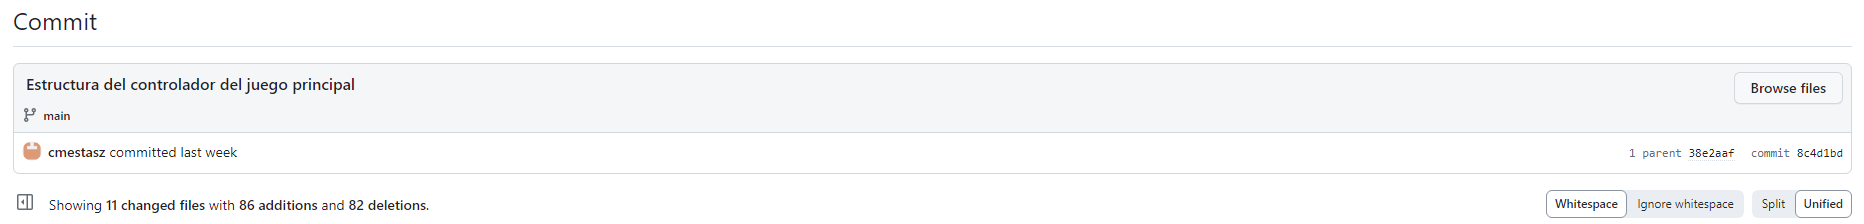
\includegraphics[width=1\textwidth,keepaspectratio]{img/commit_11.png}
	\caption{Estructura del controlador del juego principal}
\end{figure}
\begin{figure}[H]
	\centering
	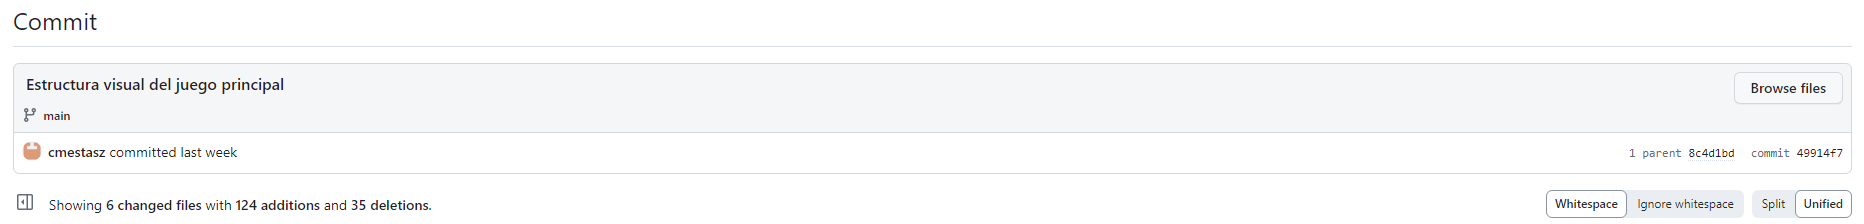
\includegraphics[width=1\textwidth,keepaspectratio]{img/commit_12.png}
	\caption{Estructura visual del juego principal}
\end{figure}
\begin{figure}[H]
	\centering
	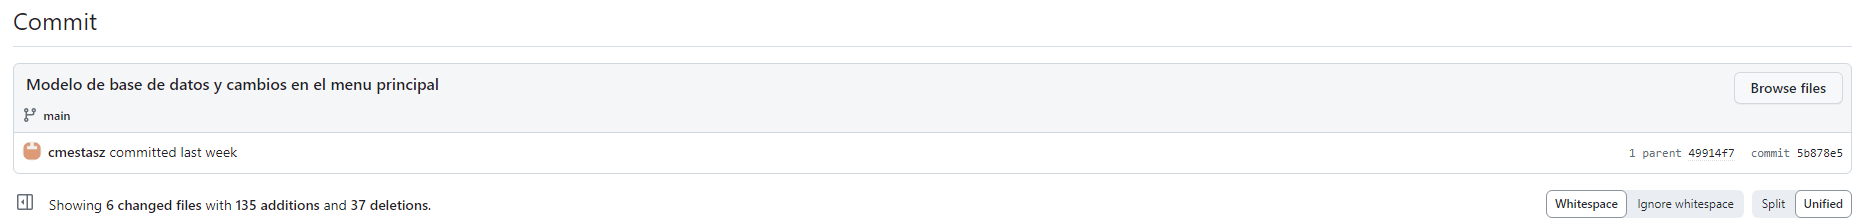
\includegraphics[width=1\textwidth,keepaspectratio]{img/commit_13.png}
	\caption{Modelo de base de datos y cambios en el menu principal}
\end{figure}
\begin{figure}[H]
	\centering
	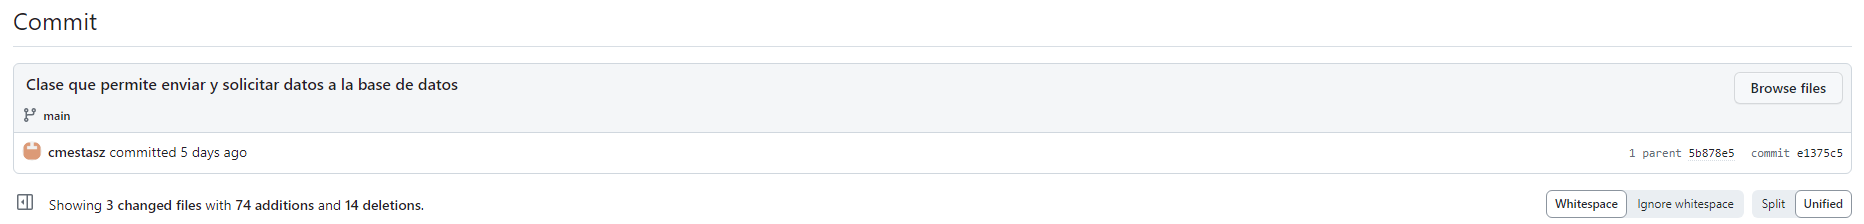
\includegraphics[width=1\textwidth,keepaspectratio]{img/commit_14.png}
	\caption{Clase que permite enviar y solicitar datos a la base de datos}
\end{figure}
\begin{figure}[H]
	\centering
	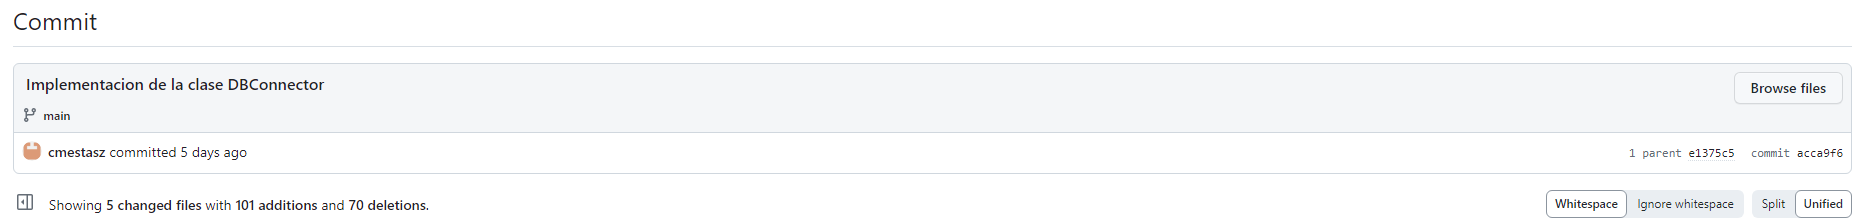
\includegraphics[width=1\textwidth,keepaspectratio]{img/commit_15.png}
	\caption{Implementacion de la clase DBConnector}
\end{figure}
\begin{figure}[H]
	\centering
	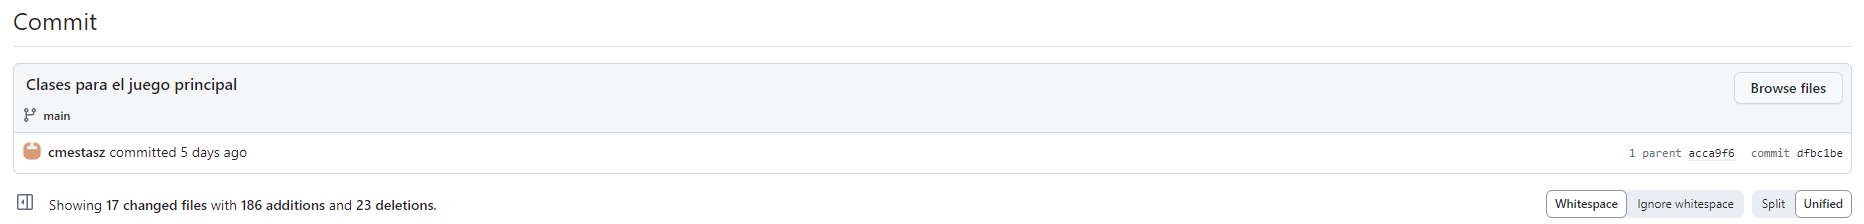
\includegraphics[width=1\textwidth,keepaspectratio]{img/commit_16.png}
	\caption{Clases para el juego principal}
\end{figure}
\begin{figure}[H]
	\centering
	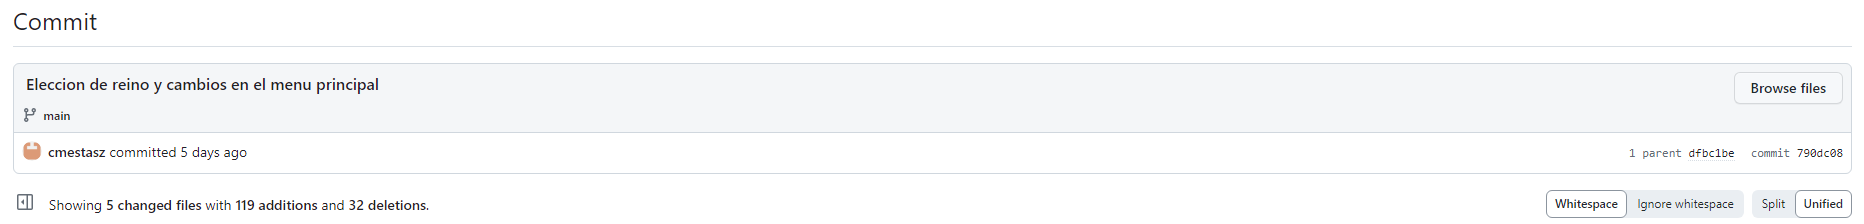
\includegraphics[width=1\textwidth,keepaspectratio]{img/commit_17.png}
	\caption{Eleccion de reino y cambios en el menu principal}
\end{figure}
\begin{figure}[H]
	\centering
	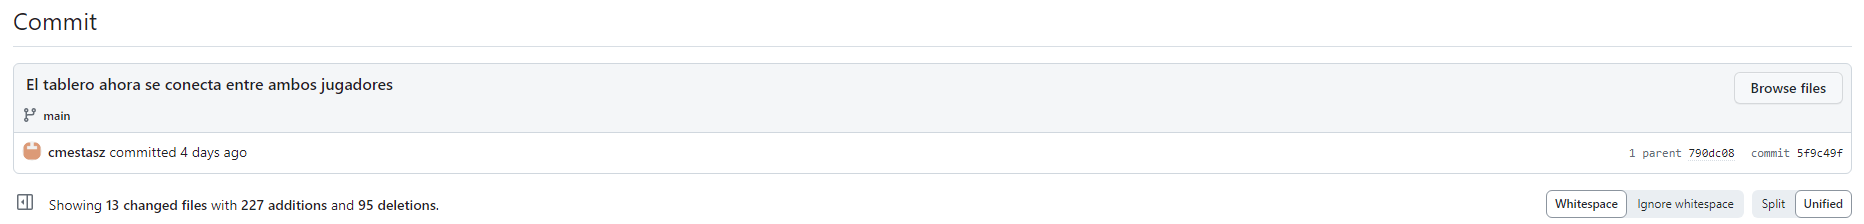
\includegraphics[width=1\textwidth,keepaspectratio]{img/commit_18.png}
	\caption{El tablero ahora se conecta entre ambos jugadores}
\end{figure}
\begin{figure}[H]
	\centering
	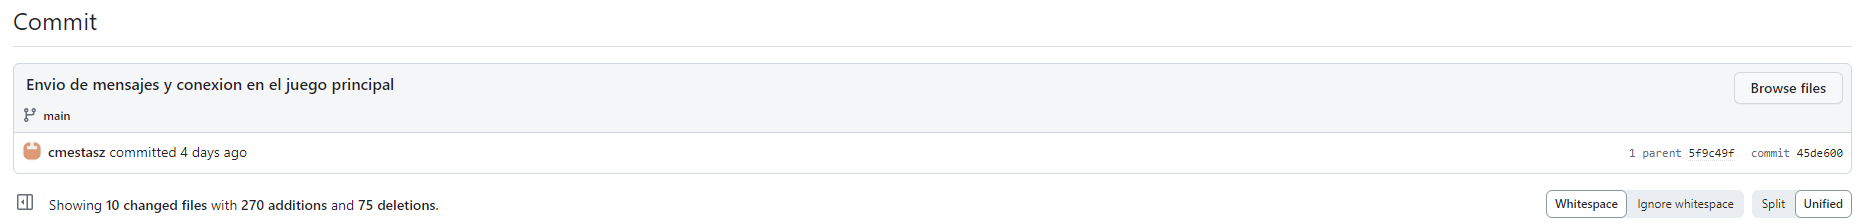
\includegraphics[width=1\textwidth,keepaspectratio]{img/commit_19.png}
	\caption{Envio de mensajes y conexion en el juego principal}
\end{figure}
\begin{figure}[H]
	\centering
	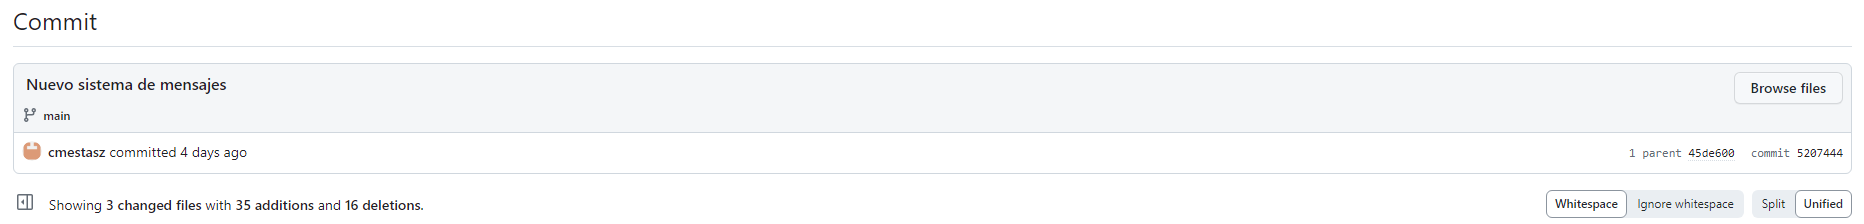
\includegraphics[width=1\textwidth,keepaspectratio]{img/commit_20.png}
	\caption{Nuevo sistema de mensajes}
\end{figure}
\begin{figure}[H]
	\centering
	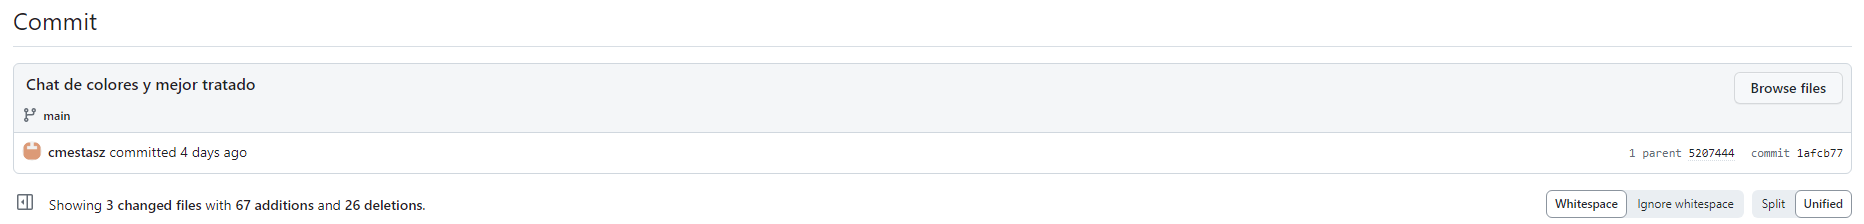
\includegraphics[width=1\textwidth,keepaspectratio]{img/commit_21.png}
	\caption{Chat de colores y mejor tratado}
\end{figure}
\begin{figure}[H]
	\centering
	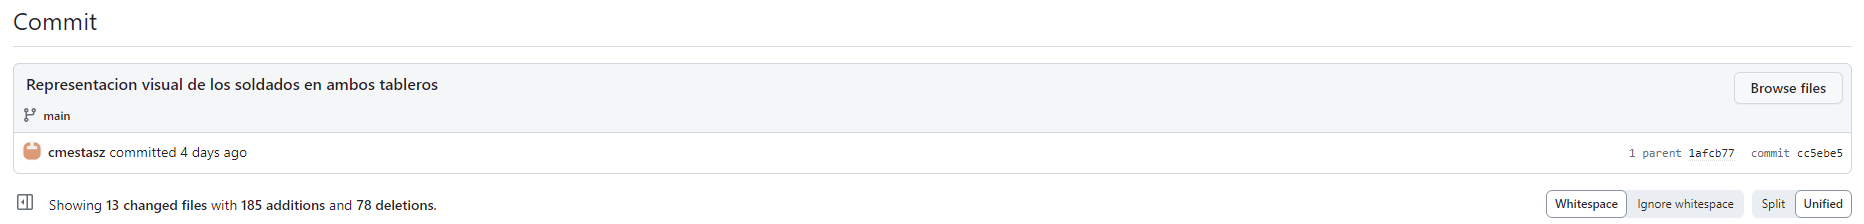
\includegraphics[width=1\textwidth,keepaspectratio]{img/commit_22.png}
	\caption{Representacion visual de los soldados en ambos tableros}
\end{figure}
\begin{figure}[H]
	\centering
	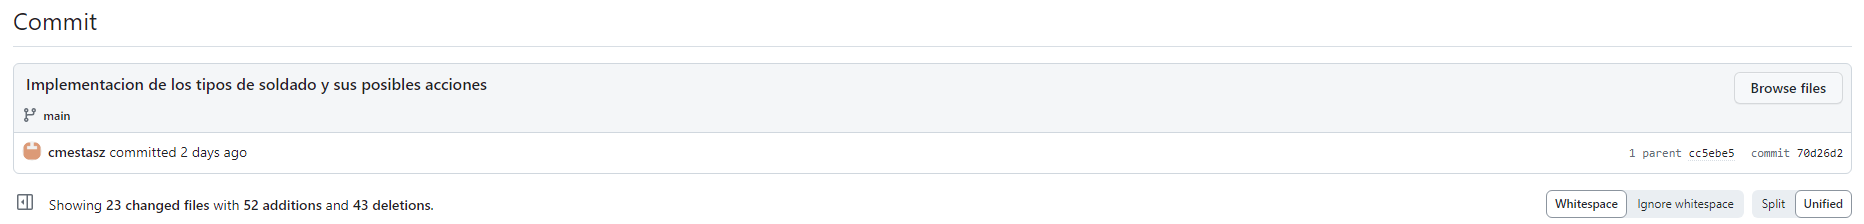
\includegraphics[width=1\textwidth,keepaspectratio]{img/commit_23.png}
	\caption{Implementacion de los tipos de soldado y sus posibles acciones}
\end{figure}
\begin{figure}[H]
	\centering
	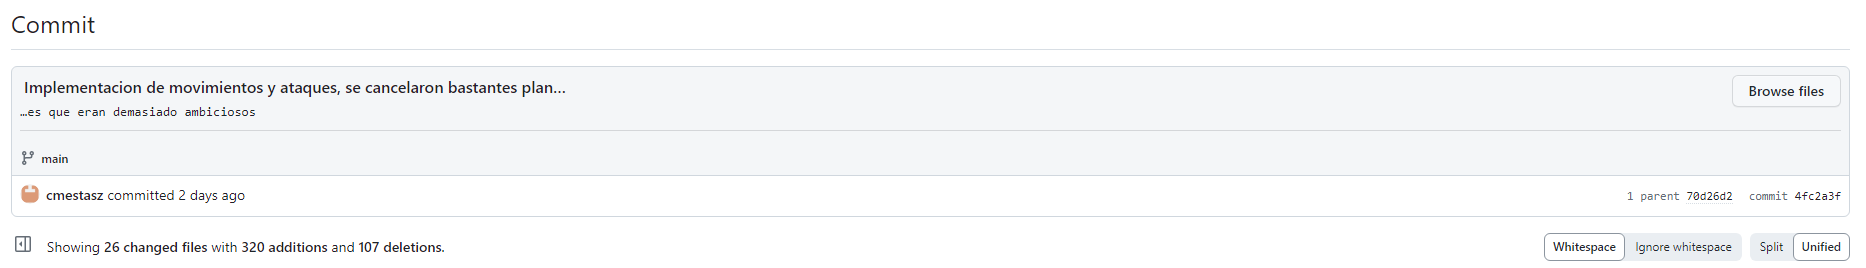
\includegraphics[width=1\textwidth,keepaspectratio]{img/commit_24.png}
	\caption{Implementacion de movimientos y ataques, se cancelaron bastantes planes que eran demasiado ambiciosos}
\end{figure}
\begin{figure}[H]
	\centering
	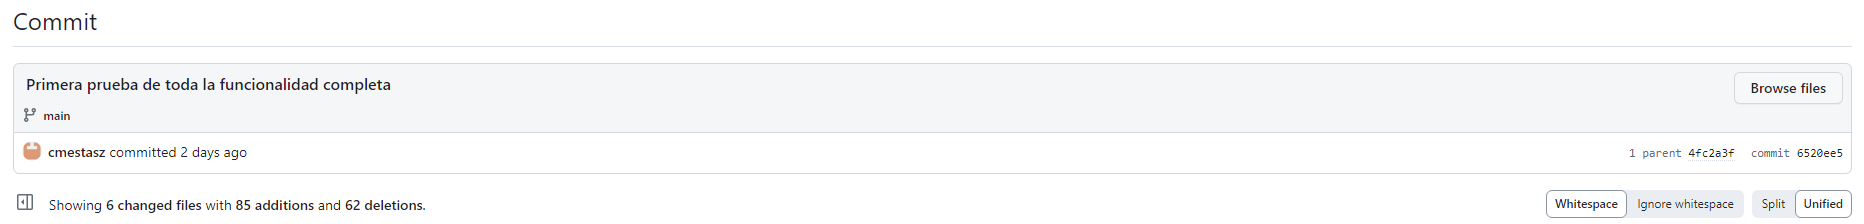
\includegraphics[width=1\textwidth,keepaspectratio]{img/commit_25.png}
	\caption{Primera prueba de toda la funcionalidad completa}
\end{figure}
\begin{figure}[H]
	\centering
	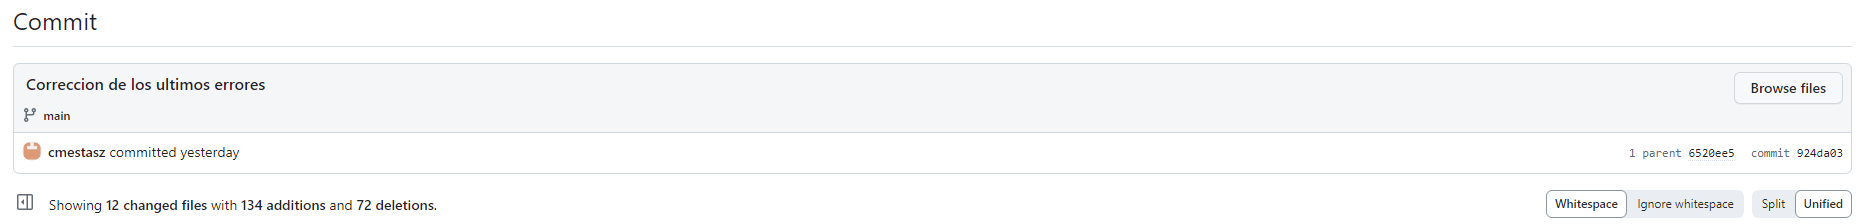
\includegraphics[width=1\textwidth,keepaspectratio]{img/commit_26.png}
	\caption{Correccion de los ultimos errores}
\end{figure}
\begin{figure}[H]
	\centering
	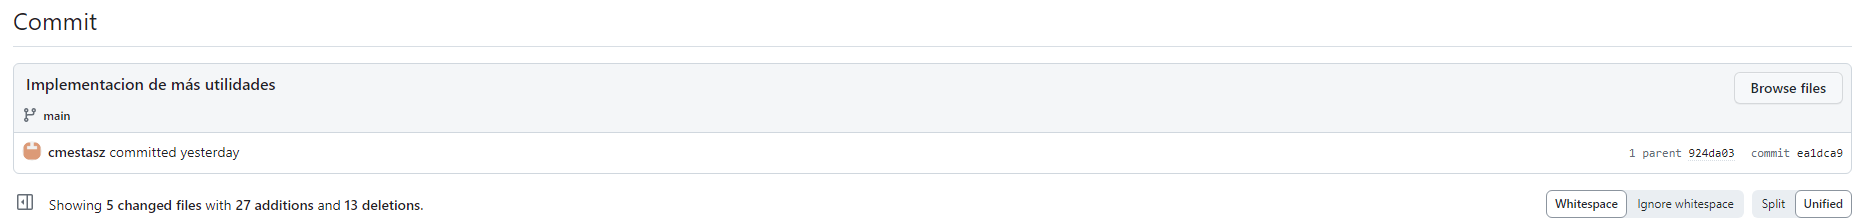
\includegraphics[width=1\textwidth,keepaspectratio]{img/commit_27.png}
	\caption{Implementacion de más utilidades}
\end{figure}
\begin{figure}[H]
	\centering
	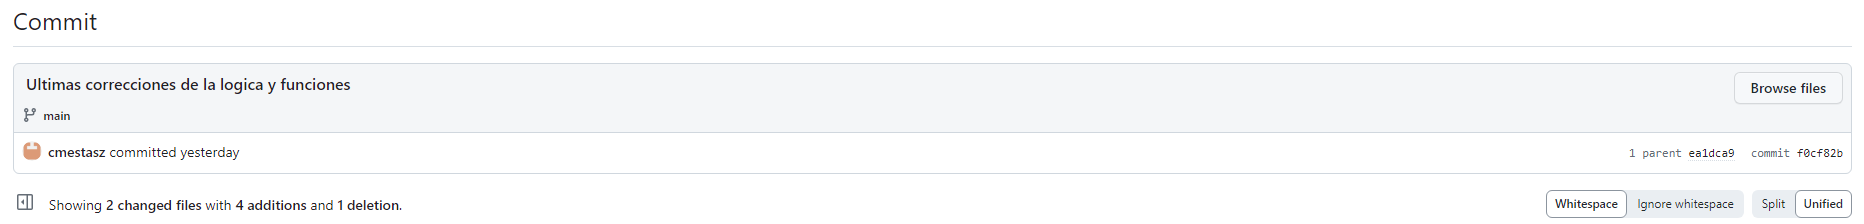
\includegraphics[width=1\textwidth,keepaspectratio]{img/commit_28.png}
	\caption{Ultimas correcciones de la logica y funciones}
\end{figure}
\begin{figure}[H]
	\centering
	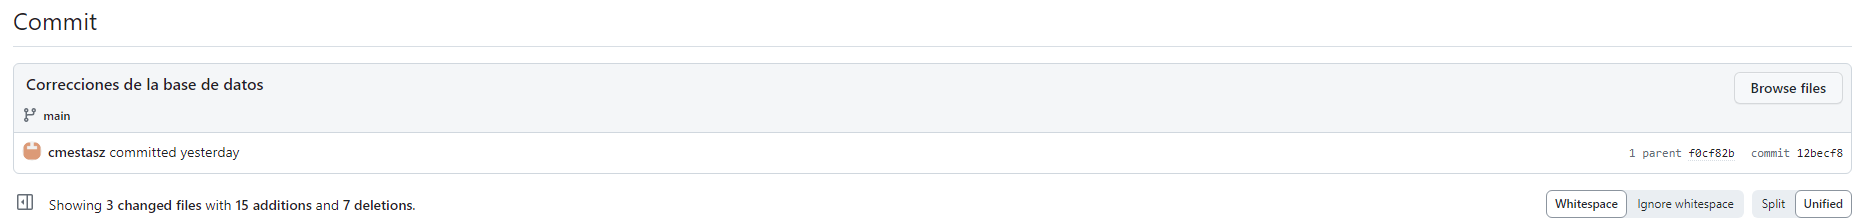
\includegraphics[width=1\textwidth,keepaspectratio]{img/commit_29.png}
	\caption{Correcciones de la base de datos}
\end{figure}
\begin{figure}[H]
	\centering
	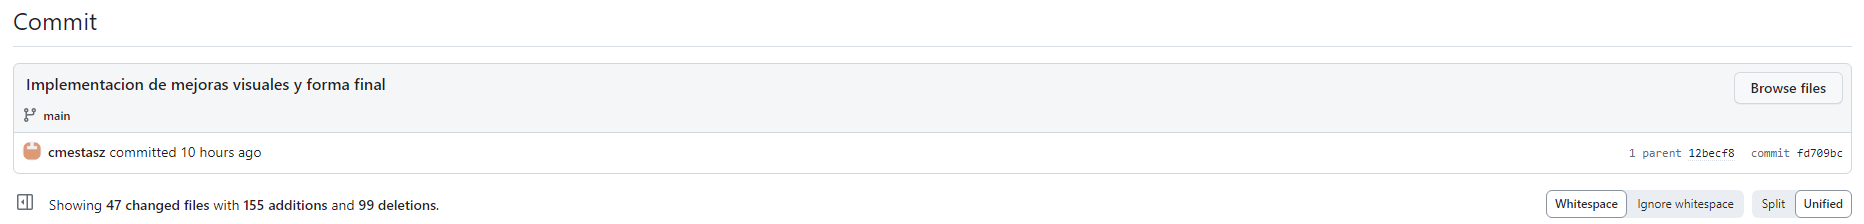
\includegraphics[width=1\textwidth,keepaspectratio]{img/commit_30.png}
	\caption{Implementacion de mejoras visuales y forma final}
\end{figure}
\begin{figure}[H]
	\centering
	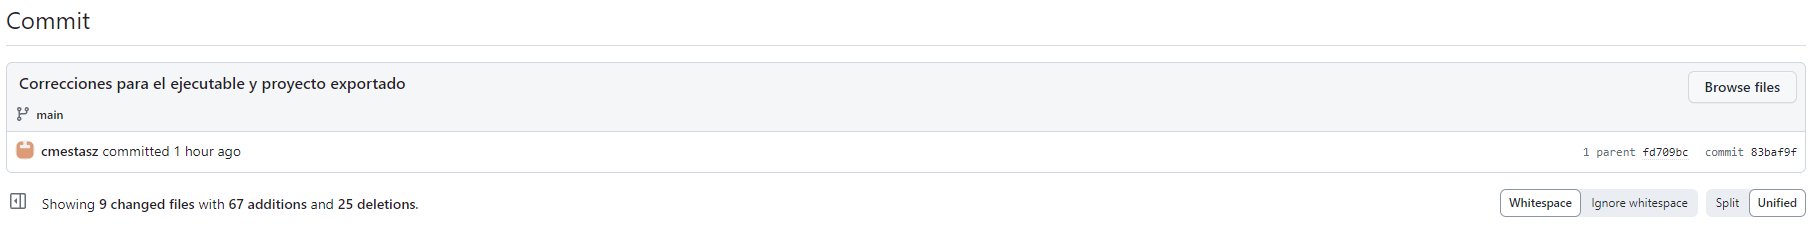
\includegraphics[width=1\textwidth,keepaspectratio]{img/commit_31.png}
	\caption{Correcciones para el ejecutable y proyecto exportado}
\end{figure}
\begin{figure}[H]
	\centering
	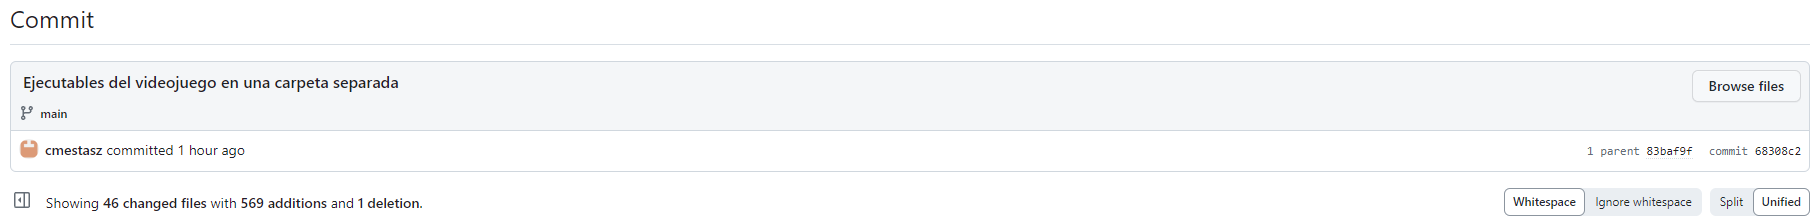
\includegraphics[width=1\textwidth,keepaspectratio]{img/commit_32.png}
	\caption{Ejecutables del videojuego en una carpeta separada}
\end{figure}
\pagebreak

\section{Código desarrollado}
\subsection{Servidor}
\lstinputlisting[language=Java, caption={MainServer.java},numbers=left,]{../SERVER/src/MainServer.java}
\begin{itemize}
	\item Clase que se encarga de recibir las peticiones de los clientes y responderlas.
	\item Al momento de abrir una instancia del videojuego, se crea una conección que se conecta con el servidor.
	\item Mediante el uso de hilos, se responde todas las peticiones de los clientes.
\end{itemize}
\lstinputlisting[language=Java, caption={DBConnector.java},numbers=left,]{../SERVER/src/Utils/DBConnector.java}
\begin{itemize}
	\item Clase que se encarga de conectarse a la base de datos y realizar las operaciones.
	\item La primera vez que se inicia, crea la base de datos y guarda el usuario que puede acceder en un archivo.
	\item Posee todos los métodos que permiten interactuar con la base de datos a lo largo de todo el juego.
\end{itemize}
\lstinputlisting[language=Java, caption={ServerConnection.java},numbers=left,]{../SERVER/src/Utils/ServerConnection.java}
\begin{itemize}
	\item Clase de utilidad para mantener una conección con el servidor.
	\item Mantiene la id de la conección, el nombre y el reino del jugador.
	\item Permite generar lectores y escritores de archivos para realizar el envio de datos.
\end{itemize}
\subsection{Videojuego}
\lstinputlisting[language=Java, caption={Archer.java},numbers=left,]{../VIDEOGAME/src/FX/MainGame/Classes/Archer.java}
\begin{itemize}
	\item Clase que almacena un arquero, y sus estadísticas.
	\item Los arqueros tiene un mayor rango de ataque.
\end{itemize}
\lstinputlisting[language=Java, caption={Knight.java},numbers=left,]{../VIDEOGAME/src/FX/MainGame/Classes/Knight.java}
\begin{itemize}
	\item Clase que almacena un caballero, y sus estadísticas.
	\item Los arqueros tiene un mayor rango de movimiento.
\end{itemize}
\lstinputlisting[language=Java, caption={Spearman.java},numbers=left,]{../VIDEOGAME/src/FX/MainGame/Classes/Spearman.java}
\begin{itemize}
	\item Clase que almacena un lancero, y sus estadísticas.
\end{itemize}
\lstinputlisting[language=Java, caption={Swordsman.java},numbers=left,]{../VIDEOGAME/src/FX/MainGame/Classes/Swordsman.java}
\begin{itemize}
	\item Clase que almacena un espadachín, y sus estadísticas.
\end{itemize}
\lstinputlisting[language=Java, caption={Soldier.java},numbers=left,]{../VIDEOGAME/src/FX/MainGame/Classes/Soldier.java}
\begin{itemize}
	\item Clase que almacena un soldado.
	\item Superclase de todas las clases de soldados.
	\item Almacena nombre, equipo, vida, ataque, defensa, y tipo.
	\item Posee métodos para simular el comportamiento de un soldado.
\end{itemize}
\lstinputlisting[language=Java, caption={Board.java},numbers=left,]{../VIDEOGAME/src/FX/MainGame/Board.java}
\begin{itemize}
	\item Clase que almacena un tablero.
	\item Almacena el terreno, los ejércitos y los reinos.
	\item Es serializable para permitir ser enviado entre ambos jugadores al momento de iniciar el juego.
\end{itemize}
\lstinputlisting[language=Java, caption={MainGameController.java},numbers=left,]{../VIDEOGAME/src/FX/MainGame/MainGameController.java}
\begin{itemize}
	\item Clase que controla el videojuego principal, se encarga de la manipulación de todos los elementos FX.
	\item Realiza la inicialización de todos los elementos del escenario.
	\item Posee métodos que permiten enviar al servidor los datos tanto de chats como de movimientos.
	\item Posee la clase interna DataReceiver que permite recibir las respuestas del servidor y ejecutarlas.
\end{itemize}
\lstinputlisting[language=XML, caption={MainGame.fxml},numbers=left,]{../VIDEOGAME/src/FX/MainGame/MainGame.fxml}
\begin{itemize}
	\item Clase FXML de JavaFX que posee el juego principal.
	\item Posee las maquetas que luego son rellenadas con el controlador para el juego principal.
\end{itemize}
\lstinputlisting[language=Java, caption={MainMenuController.java},numbers=left,]{../VIDEOGAME/src/FX/MainMenu/MainMenuController.java}
\begin{itemize}
	\item Clase que controla el menú principal, se encarga de la manipulación de todos los elementos FX.
	\item Posee métodos que permiten enviar al servidor los datos tanto de chats como de movimientos.
	\item Es el encargado de realizar la conección con la base de datos usando la clase DBConnector y con el servidor usando un archivo.
	\item Posee la clase interna DataReceiver que permite recibir las respuestas del servidor y ejecutarlas.
\end{itemize}
\lstinputlisting[language=XML, caption={MainMenu.fxml},numbers=left,]{../VIDEOGAME/src/FX/MainMenu/MainMenu.fxml}
\begin{itemize}
	\item Clase FXML de JavaFX que posee el juego principal.
	\item Posee todo el menú principal ya ordenado, puesto que el menú principal no es reescalable.
\end{itemize}
\lstinputlisting[language=Java, caption={BetterColor.java},numbers=left,]{../VIDEOGAME/src/Utils/BetterColor.java}
\begin{itemize}
	\item Clase de apoyo que contiene un color serializable.
	\item Permite generar su representación en color FX y como rgba para los estilos.
\end{itemize}
\lstinputlisting[language=Java, caption={MainGameOperation.java},numbers=left,]{../VIDEOGAME/src/Utils/MainGameOperation.java}
\begin{itemize}
	\item Interfaz que mantiene los códigos de operación y respuesta para el servidor (Del menú principal).
\end{itemize}
\lstinputlisting[language=Java, caption={MainMenuOperation.java},numbers=left,]{../VIDEOGAME/src/Utils/MainMenuOperation.java}
\begin{itemize}
	\item Interfaz que mantiene los códigos de operación y respuesta para el servidor (Del juego principal).
\end{itemize}
\lstinputlisting[language=Java, caption={Resolution.java},numbers=left,]{../VIDEOGAME/src/Utils/Resolution.java}
\begin{itemize}
	\item Clase de apoyo que contiene una resolución (ancho x alto).
\end{itemize}
\lstinputlisting[language=Java, caption={Tile.java},numbers=left,]{../VIDEOGAME/src/Utils/Tile.java}
\begin{itemize}
	\item Clase que mantiene una celda del tablero.
	\item Permite cambiar la imagen y la vida de cada celda.
	\item Posee otros métodos de utilidad como retornar posicion en el tablero y hallar distancia entre casillas.
\end{itemize}
\lstinputlisting[language=Java, caption={Utils.java},numbers=left,]{../VIDEOGAME/src/Utils/Utils.java}
\begin{itemize}
	\item Clase de utilidad que posee diferentes atajos de lectura y escritura de archivos.
\end{itemize}
\lstinputlisting[language=Java, caption={VideogameConstants.java},numbers=left,]{../VIDEOGAME/src/Utils/VideogameConstants.java}
\begin{itemize}
	\item Interfaz que mantiene valores predeterminados por el juego.
\end{itemize}
\lstinputlisting[language=Java, caption={Videogame.java},numbers=left,]{../VIDEOGAME/src/Videogame.java}
\begin{itemize}
	\item Clase principal, que instancia la ventana e inicia el juego.
\end{itemize}
\lstinputlisting[language=Java, caption={Main.java},numbers=left,]{../VIDEOGAME/src/Main.java}
\begin{itemize}
	\item Clase que llama al main de la clase principal (necesario para la exportación a jar).
\end{itemize}
\pagebreak

\section{Ejecución del código}
\subsection{Video de ejecución}
\bf{\url{https://drive.google.com/file/d/1ynmkSdxNEOvR77D_yYZbrpWrQpy3jb9m/view?usp=sharing}}
\pagebreak

\section{Diagrama UML}
\begin{figure}[H]
	\centering
	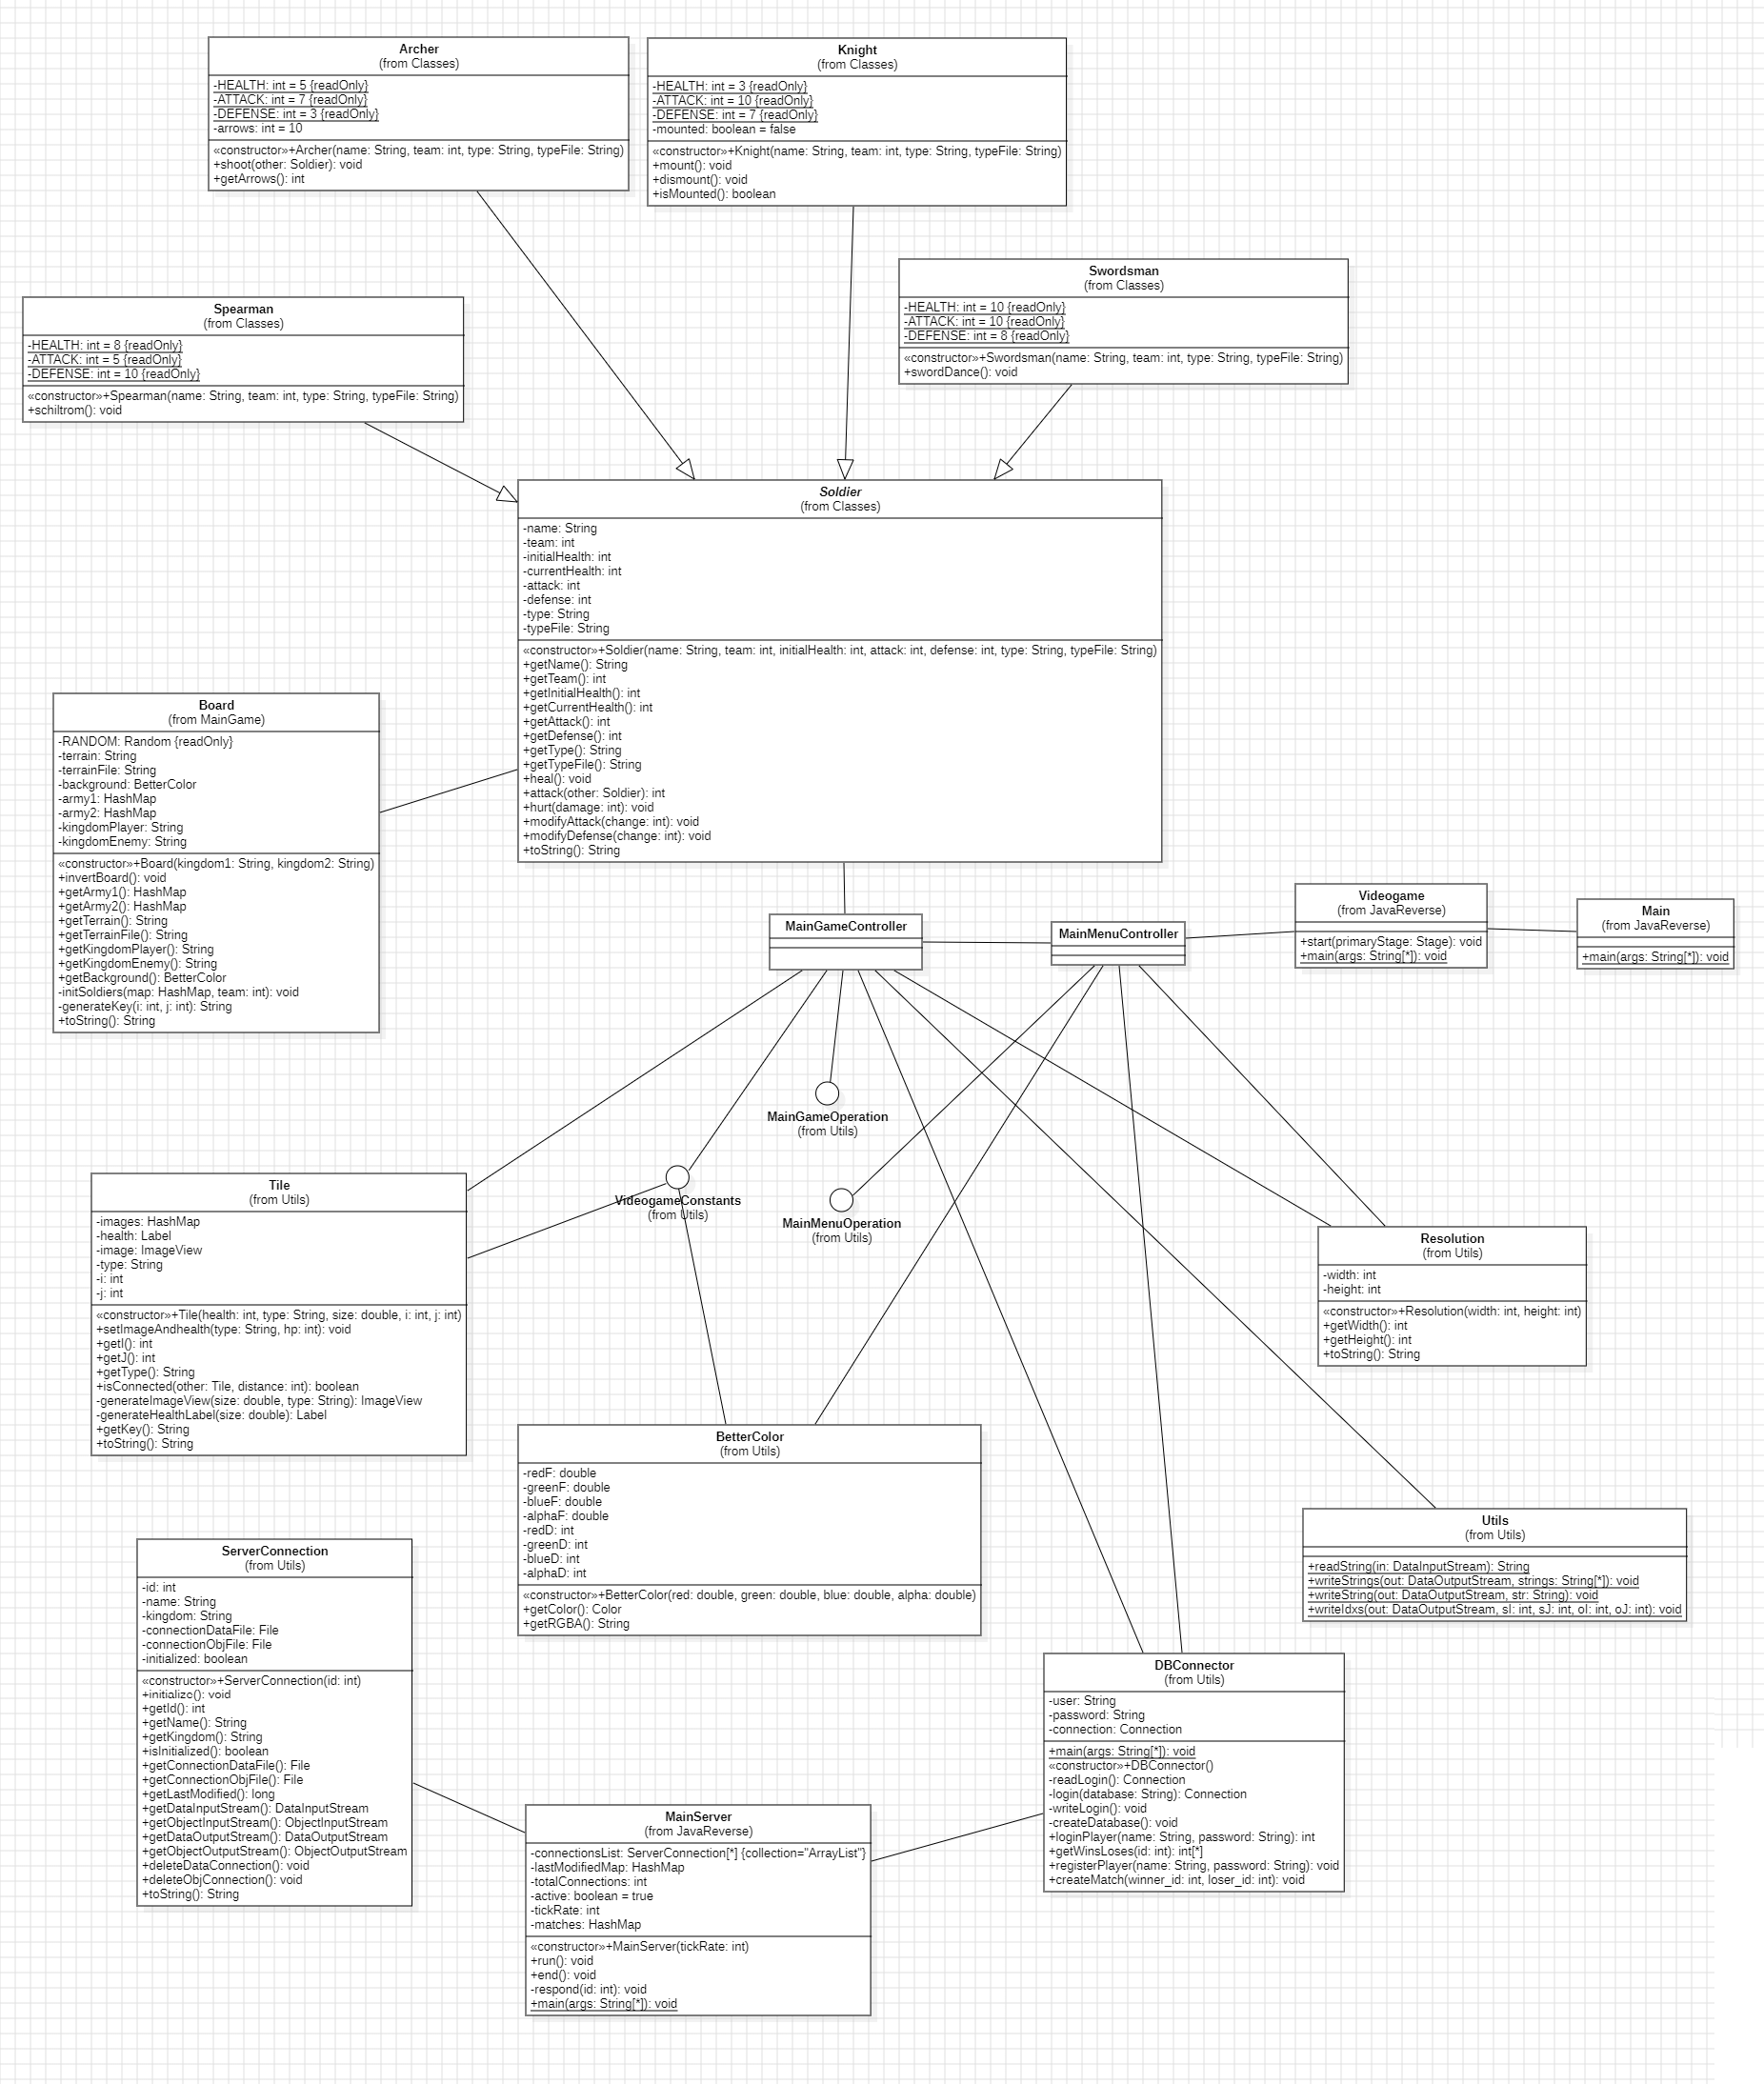
\includegraphics[width=1\textwidth,keepaspectratio]{img/uml.png}
	\caption{Diagrama UML.}
\end{figure}
\pagebreak

\section{Estructura de laboratorio \itemPracticeNumber}
\begin{itemize}
	\item El contenido que se entrega en este laboratorio es el siguiente:
\end{itemize}
%%%%%%%%%%%%%%%%%%%%%%%%%%%%%%%%%%%%%%%%%%%%%%%%%%%%%%%%%%%%%%%%%%%%%%
\begin{lstlisting}[style=ascii-tree]
proyecto_final/
|--- EJECUTABLES
	|--- SERVER.jar
	|--- VIDEOGAME.jar
|--- INFORME
	|--- img
		|--- commit_01.png
		|--- commit_02.png
		|--- commit_03.png
		|--- commit_04.png
		|--- commit_05.png
		|--- commit_06.png
		|--- commit_07.png
		|--- commit_08.png
		|--- commit_09.png
		|--- commit_10.png
		|--- commit_11.png
		|--- commit_12.png
		|--- commit_13.png
		|--- commit_14.png
		|--- commit_15.png
		|--- commit_16.png
		|--- commit_17.png
		|--- commit_18.png
		|--- commit_19.png
		|--- commit_20.png
		|--- commit_21.png
		|--- commit_22.png
		|--- commit_23.png
		|--- commit_24.png
		|--- commit_25.png
		|--- commit_26.png
		|--- commit_27.png
		|--- commit_28.png
		|--- commit_29.png
		|--- commit_30.png
		|--- commit_31.png
		|--- commit_32.png
		|--- logo_abet.png
		|--- logo_unsa.jpg
		|--- logo_episunsa.png
		|--- uml.png
	|--- commits.bash
	|--- Informe.pdf
	|--- Informe.tex
|--- SERVER
	|--- .vscode
	|--- bin
	|--- lib
	|--- src
		|--- FX
			|--- MainGame
				|--- Classes
					|--- Archer.java
					|--- Knight.java
					|--- Soldier.java
					|--- Spearman.java
					|--- Swordsman.java
				|--- Board.java
		|--- Utils
			|--- BetterColor.java
			|--- DBConnector.java
			|--- MainGameOperation.java
			|--- MainMenuOperation.java
			|--- ServerConnection.java
			|--- Utils.java
			|--- VideogameConstants.java
		|--- MainServer.java
	|--- SERVER.jar
|--- VIDEOGAME
	|--- .vscode
	|--- bin
	|--- JavaFX
	|--- lib
	|--- src
		|--- FX
			|--- MainGame
				|--- Classes
					|--- Archer.java
					|--- Knight.java
					|--- Soldier.java
					|--- Spearman.java
					|--- Swordsman.java
				|--- Board.java
				|--- MainGame.fxml
				|--- MainGameController.java
			|--- MainMenu
				|--- MainMenu.fxml
				|--- MainMenuController.java
		|--- img
			|--- action_attack.png
			|--- action_move.png
			|--- background_beach.png
			|--- background_data.png
			|--- background_desert.png
			|--- background_forest.png
			|--- background_meadow.png
			|--- background_mountain.png
			|--- settings.png
			|--- tile_archer.png
			|--- tile_knight.png
			|--- tile_spearman.png
			|--- tile_swordsman.png
			|--- tile_tile.png
			|--- waiting.png
		|--- Utils
			|--- BetterColor.java
			|--- DBConnector.java
			|--- MainGameOperation.java
			|--- MainMenuOperation.java
			|--- Resolution.java
			|--- Tile.java
			|--- Utils.java
			|--- VideogameConstants.java
		|--- Videogame.java
	|--- VIDEOGAME.jar
\end{lstlisting}
%%%%%%%%%%%%%%%%%%%%%%%%%%%%%%%%%%%%%%%%%%%%%%%%%%%%%%%%%%%%%%%%%%%%%%
\pagebreak

\section{\textcolor{red}{Rúbricas}}

\subsection{\textcolor{red}{Entregable Informe}}
\begin{table}[H]
	\caption{Tipo de Informe}
	\setlength{\tabcolsep}{0.5em} % for the horizontal padding
	{\renewcommand{\arraystretch}{1.5}% for the vertical padding
		\begin{tabular}{|M{3cm}|M{12cm}|}
			\hline
			\multicolumn{2}{|c|}{\textbf{\textcolor{red}{Informe}}}                                                                                                      \\
			\hline
			\textbf{\textcolor{red}{Latex}} & \textcolor{blue}{El informe está en formato PDF desde Latex,  con un formato limpio (buena presentación) y facil de leer.} \\
			\hline
		\end{tabular}
	}
\end{table}

\subsection{\textcolor{red}{Rúbrica para el contenido del Informe y demostración}}
\begin{itemize}
	\item El alumno debe marcar o dejar en blanco en celdas de la columna \textbf{Checklist} si cumplio con el ítem correspondiente.
	\item Si un alumno supera la fecha de entrega, su calificación será sobre la nota mínima aprobatoria, siempre y cuando cumpla con todos los items.
	\item El alumno debe autocalificarse en la columna \textbf{Estudiante} de acuerdo a la siguiente tabla:

	      \begin{table}[ht]
		      \caption{Niveles de desempeño}
		      \begin{center}
			      \begin{tabular}{ccccc}
				      \hline
				                      & \multicolumn{4}{c}{Nivel}                                                              \\
				      \cline{1-5}
				      \textbf{Puntos} & Insatisfactorio 25\%      & En Proceso 50\% & Satisfactorio 75\% & Sobresaliente 100\% \\
				      \textbf{2.0}    & 0.5                       & 1.0             & 1.5                & 2.0                 \\
				      \textbf{4.0}    & 1.0                       & 2.0             & 3.0                & 4.0                 \\
				      \hline
			      \end{tabular}
		      \end{center}
	      \end{table}

\end{itemize}

\begin{table}[H]
	\caption{Rúbrica para contenido del Informe y demostración}
	\setlength{\tabcolsep}{0.5em} % for the horizontal padding
	{\renewcommand{\arraystretch}{1.5}% for the vertical padding
		%\begin{center}
		\begin{tabular}{|M{2.3cm}|M{5cm}|M{1.2cm}|M{1.5cm}|M{1.8cm}|M{1.4cm}|}
			\hline
			\multicolumn{2}{|c|}{Contenido y demostración} & Puntos                                                                                                                                                                                                        & Checklist & Estudiante & Profesor   \\
			\hline
			\textbf{1. GitHub}                             & Hay enlace URL activo del directorio para el laboratorio hacia su repositorio GitHub con código fuente terminado y fácil de revisar.                                                                          & 2         & X          & 2        & \\
			\hline
			\textbf{2. Commits}                            & Hay capturas de pantalla de los commits más importantes con sus explicaciones detalladas. (El profesor puede preguntar para refrendar calificación).                                                          & 4         & X          & 4        & \\
			\hline
			\textbf{3. Código fuente}                      & Hay porciones de código fuente importantes con numeración y explicaciones detalladas de sus funciones.                                                                                                        & 2         & X          & 1.5      & \\
			\hline
			\textbf{4. Ejecución}                          & Se incluyen ejecuciones/pruebas del código fuente explicadas gradualmente.                                                                                                                                    & 2         & X          & 1.5      & \\
			\hline
			\textbf{5. Pregunta}                           & Se responde con completitud a la pregunta formulada en la tarea. (El profesor puede preguntar para refrendar calificación).                                                                                   & 2         & X          & 2        & \\
			\hline
			\textbf{6. Fechas}                             & Las fechas de modificación del código fuente estan dentro de los plazos de fecha de entrega establecidos.                                                                                                     & 2         & X          & 2        & \\
			\hline
			\textbf{7. Ortografía}                         & El documento no muestra errores ortográficos.                                                                                                                                                                 & 2         & X          & 1.5      & \\
			\hline
			\textbf{8. Madurez}                            & El Informe muestra de manera general una evolución de la madurez del código fuente,  explicaciones puntuales pero precisas y un acabado impecable. (El profesor puede preguntar para refrendar calificación). & 4         & X          & 4        & \\
			\hline
			\multicolumn{2}{|c|}{\textbf{Total}}           & 20                                                                                                                                                                                                            &           & 18.5       &            \\
			\hline
		\end{tabular}
		%\end{center}
		%\label{tab:multicol}
	}
\end{table}

\section{Referencias}
\begin{itemize}
	\item Aedo, M. y Castro, E. (2021). FUNDAMENTOS DE PROGRAMACIÓN 2 - Tópicos de Programación Orientada a Objetos. Editorial UNSA.
	\item JavaFX (2023). Getting Started with JavaFX. \url{https://openjfx.io/openjfx-docs/}
\end{itemize}

%\pagebreak
%\bibliographystyle{apalike}
%\bibliographystyle{IEEEtranN}
%\bibliography{bibliography}

\end{document}